\documentclass{article}
\usepackage{fontspec}
\usepackage{type1cm}
\usepackage{geometry}
\usepackage{graphicx}
\usepackage[bold-style=ISO]{unicode-math}
\usepackage[heading=true]{ctex}%添加heading=true,使用中文版式
\geometry{a4paper,left=1cm,right=1cm,top=3cm,bottom=3cm}
\usepackage{titlesec} %自定义多级标题格式的宏包
\titleformat{\section}[block]{\Huge\bfseries}{\arabic{section}}{1em}{}[]
\titleformat{\subsection}[block]{\huge\bfseries}{\arabic{section}.\arabic{subsection}}{1em}{}[]
\titleformat{\paragraph}[block]{\LARGE\bfseries}{[\arabic{paragraph}]}{1em}{}[]

\begin{document}
\begin{flushleft}
	\LARGE
	
	\section{公式}
	
	\subsection{定积分}
	
	定积分是一个特殊的极限\\
	$\int_{a}^{b}f(x)dx=\lim\limits_{\lambda\to 0}\sum_{i=1}^{n}f(\xi_i)\Delta x_i$\\
	其中$\lambda = max\{\Delta x_1, \Delta x_2...\Delta x_n\}$\\
	\ \ $\Delta x_i=x_i-x_{i-1}$\\
	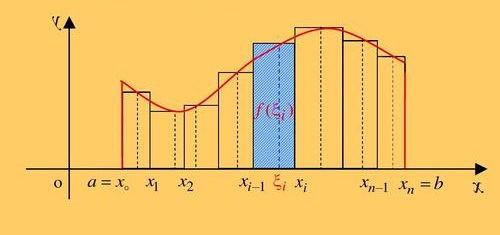
\includegraphics[scale=1.0]{2.jpg}\\
	~\\
	定积分的几何意义:曲边梯形的面积的代数和\\
	~\\
	若$f(x)$在$[a,b]$上连续,则$f(x)$在$[a,b]$上可积\\
	若$f(x)$在$[a,b]$上有界,且只有有限个间断点,则$f(x)$在$[a,b]$上可积\\
	
	\subsection{定积分的性质}
	
	1、等式性质\\
	\ \ $\int_{a}^{a}f(x)dx=0$\\
	\ \ $\int_{a}^{b}f(x)dx=-\int_{b}^{a}f(x)dx$\\
	\ \ $\int_{a}^{b}[\alpha f(x)\pm \beta g(x)]dx=\alpha\int_{a}^{b}f(x)dx\pm \beta\int_{a}^{b}g(x)dx$\\
	\ \ $\int_{a}^{b}f(x)dx=\int_{a}^{c}f(x)dx+\int_{c}^{b}f(x)dx$\\
	2、不等式性质(前提$b>a$)\\
	\ \ 设$f(x)\le g(x)$,则$\int_{a}^{b}f(x)dx\le \int_{a}^{b}g(x)dx$\\
	\ \ 设$f(x)\ge 0$,则$\int_{a}^{b}f(x)dx \ge 0$\\
	\ \ $|\int_{a}^{b}f(x)dx| \le \int_{a}^{b}|f(x)|dx$\\
	\ \ 设$m<f(x)<M$,则$m(b-a)<\int_{a}^{b}f(x)dx<M(b-a)$\\
	3、积分中值定理\\
	设$f(x)$在$[a,b]$上连续,则$\exists \xi \in [a,b]$或$\exists \xi \in (a,b)$,使得$\int_{a}^{b}f(x)dx=f(\xi)(b-a)$\\
	~\\
	使用定积分定义求极限:$\int_{0}^{1}f(x)dx=\lim\limits_{x\to \infty}\frac{1}{n}\sum_{i=1}^{n}f(\frac{i}{n})$\\
	
	\subsection{微积分基本公式}
	
	\paragraph{变上限积分函数}
	设$f(x)$在$[a,b]$上可积,$\forall x_0\in [a,b]$,$F(x)=\int_{x_0}^{x}f(t)dt,(a\le x\le b)$称为变上限积分函数\\
	\paragraph{变上限积分函数的性质}
	1、设$f(x)$在$[a,b]$上可积,则$F(x)$在$[a,b]$上连续\\
	2、设$f(x)$在$[a,b]$上连续,则$F(x)$在$[a,b]$上可导,且$F'(x)=(\int_{x_0}^{x}f(t)dt)'=f(x)$\\
	3、设$f(x)$在$[a,b]$上连续,$F(x)=\int_{x_0}^{\phi(x)}f(t)dt$,则$F'(x)=f[\phi(x)]\phi'(x)$\\
	4、设$f(x)$在$[a,b]$上连续,$F(x)=\int_{\Phi(x)}^{\phi(x)}f(t)dt$,则$F'(x)=f[\phi(x)]\phi'(x)-f[\Phi(x)]\Phi'(x)$\\
	~\\
	设$f(x)$是连续的奇(偶)函数,则$\int_{0}^{x}f(t)dt$是偶(奇)函数\\
	推广\\
	设$f(x)$是连续的奇函数,则$\forall a$都有$\int_{a}^{x}f(t)dt$是偶函数\\
	设$f(x)$是连续的偶函数,则只有$\int_{0}^{x}f(t)dt$是奇函数\\
	\paragraph{重要不等式}
	$a+b\ge 2\sqrt{ab}$\\
	\paragraph{柯西不等式}
	设$f(x)$和$g(x)$在$[a,b]$上连续,则$[\int_{a}^{b}f(x)g(x)dx]^2\le \int_{a}^{b}f^2(x)dx\int_{a}^{b}g^2(x)dx$\\
	\paragraph{牛顿-莱布尼兹公式}
	若$F(x)$是连续函数$f(x)$在$[a,b]$上的一个原函数,则$\int_{a}^{b}f(x)dx=F(b)-F(a)$\\
	
	\subsection{换元积分法}
	
	设$f(x)$在$[a,b]$上连续,且$x=\phi(t)$满足:\\
	1、$\phi(\alpha)=a$且$\phi(\beta)=b$\\
	2、$\phi(t)$在$[\alpha,\beta]$或$[\beta,\alpha]$上有连续导数,且$a\le \phi(t)\le b$\\
	则$\int_{a}^{b}f(x)dx=\int_{\alpha}^{\beta}f[\phi(t)]d\phi(t)=\int_{\alpha}^{\beta}f[\phi(t)]\phi'(t)dt$\\
	~\\
	\paragraph{常用的换元}
	$\frac{1}{x}dx=dlnx$\\
	$\frac{1}{\sqrt{x}}dx=d2\sqrt{x}$\\
	$\frac{1}{x^2}dx=d(-\frac{1}{x})$\\
	~\\
	如果被积函数都是由$\sin$或$\cos$组成,则:\\
	1、若$f(-\sin x,\cos x)=-f(\sin x,\cos x)$,则凑$d\cos x$\\
	2、若$f(\sin x,-\cos x)=-f(\sin x,\cos x)$,则凑$d\sin x$\\
	3、若$f(-\sin x,-\cos x)=f(\sin x,\cos x)$,则凑$d\tan x$\\
	\paragraph{三角代换}
	$\sqrt{a^2-x^2} \Rightarrow x=a\sin t, -\frac{\pi}{2}<t<\frac{\pi}{2}$\\
	$\sqrt{a^2+x^2} \Rightarrow x=a\tan t, -\frac{\pi}{2}<t<\frac{\pi}{2}$\\
	$\sqrt{x^2-a^2} \Rightarrow x=a\sec t, 0<t<\frac{\pi}{2}$\\
	\paragraph{根式代换}
	$\sqrt[n]{ax+b} \Rightarrow t$\\
	$\sqrt[n]{\frac{ax+b}{cx+d}} \Rightarrow t$\\
	\paragraph{倒代换}
	若被积函数分母的次方比分子的次方高两次及以上,则代换为$x=\frac{1}{t}$\\
	
	\subsection{分部积分法}
	
	$\int_{a}^{b}udv=uv|_b^a-\int_{a}^{b}vdu$\\
	\paragraph{何时用}
	两类不同的函数相乘做积分\\
	1、$P_n(x)$作$u \left\{
	\begin{array}{lcl}
	\int_{a}^{b} P_n(x)e^{ax}dx\\
	\int_{a}^{b} P_n(x)\sin axdx\\
	\int_{a}^{b} P_n(x)\cos axdx
	\end{array} \right.$\\
	2、$P_n(x)$作$v \left\{
	\begin{array}{lcl}
	\int_{a}^{b} P_n(x)lnxdx\\
	\int_{a}^{b} P_n(x)\arcsin axdx\\
	\int_{a}^{b} P_n(x)\arctan axdx
	\end{array} \right.$\\
	3、均可作$u \left\{
	\begin{array}{lcl}
	\int_{a}^{b} e^{ax}\sin \beta xdx\\
	\int_{a}^{b} e^{ax}\cos \beta xdx
	\end{array} \right.$\\
	
	\subsection{重要公式}
	
	1、若$f(x)$在$[-a,a]$上连续,则$\int_{-a}^{a}f(x)dx=\int_{0}^{a}[f(x)+f(-x)]dx$\\
	2、若$f(x)$在$[-a,a]$上连续,则$\int_{-a}^{a}f(x)dx=\left\{
	\begin{array}{lcl}
	2\int_{0}^{a}f(x)dx, & f(x)\mbox{为偶函数}\\
	0, & f(x)\mbox{为奇函数}
	\end{array} \right.$\\
	3、若$f(x)$是连续函数且周期为T,则:\\
	\ \ (1)$\int_{a}^{a+T}f(x)dx=\int_{-\frac{T}{2}}^{\frac{T}{2}}f(x)dx=\int_{0}^{T}f(x)dx$\\
	\ \ (2)$\int_{a}^{a+nT}f(x)dx=n\int_{0}^{T}f(x)dx$\\
	只要相差一个周期就相等\\
	4、若$f(x)$在$[0,1]$上连续,则:\\
	\ \ (1)$\int_{0}^{\frac{\pi}{2}}f(sinx)dx=\int_{0}^{\frac{\pi}{2}}f(cosx)dx$\\
	\ \ (2)$\int_{0}^{\pi}xf(sinx)dx=\frac{\pi}{2}\int_{0}^{\pi}f(sinx)dx$\\
	5、$\int_{a}^{b}\frac{1}{1+e^t}dt=\int_{a}^{b}(\frac{1}{1+e^t}\frac{e^{-t}}{e^{-t}})dt=-\int_{a}^{b}\frac{d(e^{-t}+1)}{e^{-t}+1}=-ln(e^{-t}+1)|_a^b$\\
	6、华里氏公式:$\int_{0}^{\frac{\pi}{2}}sin^nxdx=\int_{0}^{\frac{\pi}{2}}cos^nxdx=\left\{
	\begin{array}{lcl}
	\frac{n-1}{n}\frac{n-3}{n-2}...\frac{2}{3}, & n\mbox{是大于1的奇数}\\
	\frac{n-1}{n}\frac{n-3}{n-2}...\frac{1}{2}\frac{\pi}{2}, & n\mbox{是偶数}
	\end{array} \right.$\\
	示例:\\
	\ \ $\int_{0}^{\frac{\pi}{2}}sin^5xdx=\frac{4}{5}\times\frac{2}{3}=\frac{8}{15}$\\
	\ \ $\int_{0}^{\frac{\pi}{2}}cos^6xdx=\frac{5}{6}\times\frac{3}{4}\times\frac{1}{2}\times\frac{\pi}{2}=\frac{8}{15}$\\
	
	\subsection{反常积分}
	
	设$F(x)$是$f(x)$在相应区间上的一个原函数:\\
	1、$\int_{a}^{+\infty}f(x)dx=\lim\limits_{x\to+\infty}F(x)-F(a)$\\
	\ \ 若上述极限存在,则称反常积分收敛,否则发散\\
	2、$\int_{-\infty}^{b}f(x)dx=F(b)-\lim\limits_{x\to-\infty}F(x)$\\
	\ \ 若上述极限存在,则称反常积分收敛,否则发散\\
	3、$\int_{-\infty}^{+\infty}f(x)dx=\int_{-\infty}^{x_0}f(x)dx+\int_{x_0}^{+\infty}f(x)dx$\\
	\ \ 若右端的积分都收敛,则称反常积分收敛,否则发散\\
	~\\
	设$F(x)$是$f(x)$在相应区间上的一个原函数:\\
	1、若$x=a$是瑕点,则$\int_{a}^{b}f(x)dx=F(b)-\lim\limits_{x\to a^+}F(x)$\\
	\ \ 若上述极限存在,则称反常积分收敛,否则发散\\
	2、若$x=b$是瑕点,则$\int_{a}^{b}f(x)dx=\lim\limits_{x\to b^-}F(x)-F(a)$\\
	\ \ 若上述极限存在,则称反常积分收敛,否则发散\\
	3、若$c\in(a,b)$是瑕点,则$\int_{a}^{b}f(x)dx=\int_{a}^{c}f(x)dx+\int_{c}^{b}f(x)dx$\\
	\ \ 若右端的积分都收敛,则称反常积分收敛,否则发散\\
	~\\
	瑕点:使$f(x)$无界的点\\
	
	\subsection{重要结论}
	
	1、$\int_{a}^{+\infty}\frac{dx}{x^p}\left\{
	\begin{array}{lcl}
	p>1, & \mbox{收敛}\\
	p\le 1, & \mbox{发散}
	\end{array} \right.(a>0)$\\
	2、$\int_{a}^{+\infty}\frac{dx}{x(lnx)^p}\left\{
	\begin{array}{lcl}
	p>1, & \mbox{收敛}\\
	p\le 1, & \mbox{发散}
	\end{array} \right.(a>1)$\\
	3、$\int_{a}^{+\infty}x^ke^{-\lambda x}dx\left\{
	\begin{array}{lcl}
	\lambda>0, & \mbox{收敛}\\
	\lambda\le 0, & \mbox{发散}
	\end{array} \right.(k\ge 0)$\\
	4、$\int_{a}^{b}\frac{dx}{(x-a)^p}\left\{
	\begin{array}{lcl}
	p>1, & \mbox{收敛}\\
	p\le 1, & \mbox{发散}
	\end{array} \right.$\\
	5、泊松积分:$\int_{0}^{+\infty}e^{-x^2}dx=\frac{\sqrt{\pi}}{2}$\\
	6、$\lim\limits_{x\to 0^+}xlnx=0$\\
	~\\
	设$f(x)$在$(-\infty,+\infty)$内连续且是偶函数,若$\int_{0}^{+\infty}f(x)dx$收敛,则$\int_{-\infty}^{+\infty}f(x)dx=2\int_{0}^{+\infty}f(x)dx$\\
	
\end{flushleft}
\end{document}